% \documentclass{standalone}

% \input{../tikz_header}

% \begin{document}


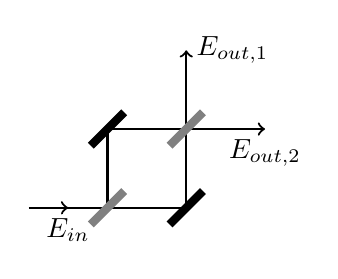
\begin{tikzpicture}[BS style/.style={draw=gray, line width=3pt},
    mirror style/.style={draw=black, line width=3pt},]
    %\useasboundingbox (-2.5,-1.5) rectangle (3,2.3);
    %\draw (-2.5,-1.5) rectangle (3,2.3);
 
    \pgfmathsetmacro{\len}{0.3}


    \coordinate (BS1) at (0,0);
    \coordinate (BS2) at (1,1);
    \coordinate (m1) at (1,0);
    \coordinate (m2) at (0,1);
    \coordinate (in) at (-1,0);
    \coordinate (out1) at (1,2);
    \coordinate (out2) at (2,1);

    \draw[thick, -> ] (in) -- (m1) -- (out1) node[right] {$E_{out,1}$};
    \draw[thick, -> ] (in) -- ++(0:0.5) node[below] {$E_{in}$};

    \draw[thick, -> ] (BS1) -- (m2) -- (out2) node[below] {$E_{out,2}$};

    \draw[style=BS style] (BS1) ++ (45:\len) -- ++(-135:{2*\len});
    \draw[style=BS style] (BS2) ++ (45:\len) -- ++(-135:{2*\len});
    \draw[style=mirror style] (m2) ++ (45:\len) -- ++(-135:{2*\len});
    \draw[style=mirror style] (m1) ++ (45:\len) -- ++(-135:{2*\len});
   


\end{tikzpicture}


%\end{document}